\documentclass[11pt,a4paper]{article}
\usepackage[margin=2.2cm]{geometry}
\usepackage[T1]{fontenc}
\usepackage{lmodern}
\usepackage{amsmath,amssymb}
\usepackage{booktabs}
\usepackage{graphicx}
\usepackage{float}
\usepackage{xcolor}
\usepackage{caption}
\usepackage{enumitem}
\usepackage[colorlinks=true,linkcolor=blue!50!black,citecolor=blue!50!black,urlcolor=blue!50!black]{hyperref}

\captionsetup{font=small,labelfont=bf}
\setlist{itemsep=2pt,topsep=4pt}
\newcommand{\dmtl}{\Delta_{\text{MTL}}}
\newcommand{\mae}{MAE$_{\log}$}

\title{Federated Learning for Heterogeneous and Private\\Indian Judicial Data}
\author{Bijinepalli Surat Dhani (23087) \and Poorvai Chandrasen \and Palak Kumari (23217) \and Biswadeep Chakraborty (23089)\\[4pt]
\small IISER Bhopal}
\date{November 2026}

\begin{document}
\maketitle

\begin{abstract}
Court records in India are spread across High Courts that cannot easily pool them, because case
descriptions, particularly before filing, can contain sensitive information. We study whether
federated learning (FL), where each court trains on its own data and only shares model updates, can
support three prediction tasks from the text of a judgment: case duration, case type and disposal
nature. Treating five High Courts (Bombay, Delhi, Karnataka, Kerala and Madhya Pradesh) as clients,
we first show with statistical tests that the courts are strongly non-IID, mainly because the same
type of case takes a different time and ends differently in each court, and because each court
drafts judgments in its own style (a linear classifier identifies the court from masked text with
99.97\% accuracy). We then compare local, centralized and federated training, including the
algorithms benchmarked in FedLegal, using an InLegalBERT encoder with LoRA adapters, so that only
about 1\% of the model leaves a court. Standard federated algorithms (FedAvg, FedProx, FedAdam) do
not beat local training, and FedProx and FedAdam are 3--4\% worse. With per-task personalisation, which we
implement as learned per-task mixing of shared and court-specific heads, federated training improves on
local training by 3.6\% across the three tasks (Wilcoxon $p=0.015$), helps the hardest court, and is
statistically tied with centralized training on pooled data ($p=0.30$). Federation helps most for
courts with a few hundred labelled cases, and gives a court with no labelled data a better model than
any single other court in four of five cases.
\end{abstract}

% =====================================================================================
\section{Introduction}
India's courts face a backlog of tens of millions of pending cases~\cite{njdg}. A decision-support
system that reads a case description and estimates how long the case will take, what type of case it
is and how it is likely to be disposed of could help lawyers prepare cases, help registries plan
judicial resources, and make legal research faster. Building such a system needs training data from
many courts, but case descriptions can contain sensitive information, particularly before a case is
formally filed, and courts are separate institutions that may not be allowed to send their records to
a central server. Federated learning (FL)~\cite{mcmahan2017communication} offers an alternative:
each court trains the model on its own records and only sends model updates to a server, which
combines them.

FL is known to struggle when the clients' data are not identically distributed
(non-IID)~\cite{li2020federated,kairouz2021advances}. Indian High Courts differ in case mix,
procedure and drafting, and the only federated benchmark for legal text, FedLegal~\cite{zhang2023fedlegal},
found that real non-IID legal data hurt standard FL. Whether FL is useful for Indian courts therefore
has to be shown, not assumed. We simulate a federation of five High Courts using their public 2024
judgments~\cite{dattam_hc} and ask:
\begin{enumerate}[label=\textbf{RQ\arabic*}]
  \item Are the courts measurably non-IID, and in which of the three tasks?
  \item Does federated training beat what a court can do alone, how does it compare with existing
        federated algorithms, and how close does it get to centralized training on pooled data?
  \item What does federation give a court that it cannot get alone, when its own data are scarce or
        when it has no labelled data at all?
\end{enumerate}

\paragraph{Tasks.} From the text of a judgment, with its operative ending removed, the model predicts
(1) the \textbf{case duration} from registration to decision, (2) the \textbf{case type} (ten
families) and (3) the \textbf{disposal nature} (allowed, dismissed, disposed of, withdrawn). The
proposal also listed Constitutional-article prediction and past-case retrieval. We dropped them:
Article citations are rare in the High Court sample (3\% of Bombay judgments), retrieval needs a
different model and evaluation that would not share the federated encoder, and statute and precedent
retrieval on Indian data is already covered by centralized benchmarks such as IL-TUR~\cite{joshi2024iltur}.
The three remaining tasks share one input and one model, and they are the tasks on which courts differ
most.

\paragraph{Contributions.}
\begin{itemize}
  \item A statistical characterisation of how five Indian High Courts differ, covering all four kinds
        of FL heterogeneity (quantity, label, concept and covariate shift), with effect sizes.
  \item The first federated study on Indian court data: local, centralized and seven federated methods
        (FedAvg, FedProx, FedAdam, SCAFFOLD, FedPer, Ditto and ours) under the same encoder, data and
        budget, with three seeds, worst-court results and paired significance tests.
  \item Per-task learned mixing (PTM) of shared and court-specific heads, whose learned weights show,
        per court and per task, how much a court relies on collaboration.
  \item Two experiments on what federation gives a court: reduced training data, and a court held
        out of training entirely.
\end{itemize}

\paragraph{Main findings.} The courts differ mainly in how the same kind of case behaves and in how
judgments are written, more than in their label mix. Because of this, standard FL algorithms do not
beat local training. Personalising the task heads per court fixes this: federated training then beats
local training, protects the hardest court, and reaches the accuracy of centralized training without
moving any judgment.

% =====================================================================================
\section{Related Work}
\paragraph{Federated learning under heterogeneity.} FedAvg~\cite{mcmahan2017communication} averages
client models weighted by data size. FedProx~\cite{li2020federated} adds a proximal term to limit
client drift, SCAFFOLD~\cite{karimireddy2020scaffold} corrects drift with control variates, and
FedAvgM and FedAdam~\cite{hsu2019fedavgm,reddi2021adaptive} add server momentum or adaptive server
steps. Loss-based client weighting~\cite{fedlbw2026} and q-FFL~\cite{li2020qffl} reweight clients
by their loss. Personalised FL keeps part of the model per client: FedPer~\cite{arivazhagan2019fedper}
and FedRep~\cite{collins2021fedrep} keep the heads local, Ditto~\cite{li2021ditto} trains a personal
model regularised towards the global one, and APFL~\cite{deng2020apfl} and FedALA~\cite{zhang2023fedala}
blend global and local models. FedHCA$^2$~\cite{lu2024fedhca2} and task-aware FL~\cite{taskawarefl2025}
address multi-task federations. Our PTM blends a shared and a local head per \emph{task}, which matters
when tasks differ in how court-specific they are.

\paragraph{Federated legal NLP.} FedLegal~\cite{zhang2023fedlegal} is a federated benchmark of legal
NLP tasks on Chinese court data; its main conclusion is that real legal non-IID data hurt FL.
FedJudge~\cite{yue2023fedjudge} fine-tunes legal language models federatedly. Neither uses Indian data
or predicts case duration.

\paragraph{Indian legal NLP.} IL-TUR~\cite{joshi2024iltur} is the standard benchmark for Indian legal
text understanding (named-entity recognition, rhetorical roles, judgment prediction with explanation,
bail prediction, statute identification, prior-case retrieval, summarisation and translation), with
centralized training only. InLegalBERT~\cite{paul2023inlegalbert} is a BERT model pre-trained on
Indian legal text. LeSICiN~\cite{paul2022lesicin} identifies statutes with a heterogeneous graph,
Vats et al.~\cite{vats2023llms} evaluate LLMs on statute and judgment prediction, NyayaRAG~\cite{nigam2025nyayarag}
adds retrieved statutes and precedents to judgment prediction, and OpenNyAI~\cite{kalamkar2022ner}
provides legal named-entity recognition. All assume centrally pooled data and none predicts case
duration. Table~\ref{tab:novelty} summarises the difference.

\begin{table}[H]\centering\small
\begin{tabular}{@{}lccc@{}}\toprule
 & FedLegal~\cite{zhang2023fedlegal} & IL-TUR~\cite{joshi2024iltur} & This work \\ \midrule
Jurisdiction & China & India & India, 5 High Courts \\
Federated training, courts as clients & \checkmark & -- & \checkmark \\
Statistical test of heterogeneity & -- & -- & \checkmark \\
Case duration (regression) & -- & -- & \checkmark \\
Case type + disposal, multi-task & -- & -- & \checkmark \\
Judgment / outcome prediction & \checkmark & \checkmark & disposal nature \\
Per-task personalisation & -- & -- & \checkmark \\
Unseen-court evaluation & -- & -- & \checkmark \\ \bottomrule
\end{tabular}
\caption{Coverage of the closest benchmarks. IL-TUR's tasks do not overlap with ours, so its numbers
are not directly comparable; its centralized setting corresponds to our centralized baseline. The
comparison with FedLegal is made by running its kind of algorithms on our data (Table~\ref{tab:main}).}
\label{tab:novelty}
\end{table}

% =====================================================================================
\section{Data}
\paragraph{Source.} The Indian High Court Judgments dataset~\cite{dattam_hc} (eCourts, CC-BY-4.0)
gives, per case, the CNR number, title (case type and parties), judges, registration and decision
dates, disposal nature and the judgment PDF. We use all cases decided in 2024 by five High Courts,
each one federated client.

\paragraph{Cleaning.} Per CNR we keep the final order with the latest decision date and drop cases
with only interim orders, whose decision date is not the disposal date. Registration dates mix
YYYY-MM-DD and DD-MM-YYYY; parsing a single format silently discarded most Bombay and Madhya Pradesh
rows, so both are parsed explicitly. Dropping negative durations and registrations before 1980 leaves
193,339 cases (Table~\ref{tab:clients}). Each court is split by decision date into 70/15/15\%
train/validation/test, so test cases are always later than training cases.

\begin{table}[H]\centering\small
\begin{tabular}{@{}lrrrrrrrrl@{}}\toprule
 & \multicolumn{3}{c}{Cases} & Median & \multicolumn{4}{c}{Disposal time (\% of cases)} & Largest \\
\cmidrule(lr){2-4}\cmidrule(lr){6-9}
Court & Train & Val & Test & days & $\le$30d & 31--180d & 181--730d & $>$730d & family \\ \midrule
Bombay & 12,923 & 2,778 & 2,722 & 64 & 38.1 & 27.7 & 18.0 & 16.2 & Writ (33\%) \\
Delhi & 35,414 & 7,394 & 7,447 & 88 & 39.6 & 20.0 & 20.6 & 19.8 & Writ (37\%) \\
Karnataka & 40,028 & 8,668 & 8,426 & 390 & 18.6 & 20.0 & 22.5 & 38.8 & Writ (43\%) \\
Kerala & 32,163 & 6,811 & 6,808 & 65 & 37.8 & 22.9 & 11.0 & 28.3 & Writ (53\%) \\
Madhya Pradesh & 15,242 & 3,316 & 3,199 & 20 & 61.3 & 25.6 & 6.0 & 7.1 & Bail (53\%) \\ \bottomrule
\end{tabular}
\caption{Federated clients after cleaning (2024 decisions).}
\label{tab:clients}
\end{table}

\paragraph{Text sample and labels.} We extracted the text of 2,500 random judgments per court and
removed PDFs with broken font encoding (0--2.7\% per court), leaving 12,360 judgments. Labels are
derived as follows. \emph{Duration} is the number of days from registration to decision. \emph{Case
type} maps the 165 court-specific codes in the case title (e.g.\ WP, BA, CRLMC) to ten families: writ,
bail, criminal, civil, contempt, arbitration, review, tax, motor accident and other. \emph{Disposal
nature} is read from the last operative statements of the judgment, because the metadata label is
missing for every Delhi case and is spelled in 13--38 different ways elsewhere; 39\% of judgments are
\emph{disposed of}, 24\% \emph{dismissed}, 23\% \emph{allowed} and 14\% \emph{withdrawn}. Cases with
an unclear outcome are kept for the other two tasks.

\paragraph{Leakage control.} All cases were decided in 2024, so dates in the text almost reveal the
duration. We mask all dates, four-digit years and multi-digit numbers, remove the operative ending,
and mask the outcome words \emph{allowed, dismissed, disposed of, withdrawn, rejected, not pressed}
and \emph{infructuous}. A check of all masked texts found no remaining four-digit year or multi-digit
number. A few outcome-related words remain (\emph{quashed} in 13.6\% of texts, \emph{granted} 7.4\%),
mostly in what the petitioner asked for; they shift the label distribution only mildly.

\paragraph{Ethics.} All records are public. Judgments contain party and lawyer names, but names are not
used as separate features and judge identity is not an input. The models are research artefacts, not
tools for deciding individual cases.

% =====================================================================================
\section{Are the Courts Non-IID?}
\label{sec:hetero}
FL distinguishes four kinds of client heterogeneity~\cite{kairouz2021advances}: different amounts of
data (quantity skew), different label distributions $P_k(y)$ (label skew), different inputs $P_k(x)$
(covariate shift) and different input--label relations $P_k(y\mid x)$ (concept shift). We test each on
the 12,360 judgments used in the experiments (Table~\ref{tab:hetero}, Figure~\ref{fig:hetero}). The text
sample has about 2,500 judgments per court by design, so quantity skew is measured on all 284,405
decisions of 2024: the largest court has 7.5 times the cases of the smallest.

\begin{table}[H]\centering\small
\resizebox{\linewidth}{!}{\begin{tabular}{@{}llll@{}}\toprule
Kind & Test & Statistic & Effect size \\ \midrule
Label: duration & Kruskal--Wallis on $\log(1+\text{days})$ & $H=555$, $p<10^{-100}$ & $\varepsilon^2=0.045$; mean pairwise KS $D=0.21$ \\
Label: duration class & $\chi^2$, court $\times$ 4 classes & $\chi^2_{12}=743$, $p<10^{-100}$ & Cram\'er's $V=0.14$ \\
Label: case family & $\chi^2$, court $\times$ 10 families & $\chi^2_{36}=4{,}045$, $p<10^{-300}$ & $V=0.29$; mean pairwise JSD $=0.15$ \\
Label: disposal & $\chi^2$, court $\times$ 4 outcomes & $\chi^2_{12}=808$, $p<10^{-100}$ & $V=0.15$; mean pairwise JSD $=0.03$ \\
Concept: duration $\mid$ type & two-way ANOVA, court $\times$ family & $F_{12}=39.4$, $p<10^{-90}$ & $R^2$: $0.028\rightarrow0.127$ with court \\
Concept: disposal $\mid$ type & $\chi^2$ within each family & $\chi^2_{69}=1{,}648$, $p<10^{-290}$ & median $V=0.22$ (8 families) \\
Covariate: text & court identification from masked text & 99.97\% (chance 20\%) & binomial $p<10^{-300}$ \\
All: transfer & train on court $i$, test on court $j\neq i$ & \mae{} $1.32\rightarrow2.01$ & disposal F1 $0.65\rightarrow0.25$ \\ \bottomrule
\end{tabular}}
\caption{Heterogeneity tests on the 12,360 judgments. JSD: Jensen--Shannon divergence (base 2;
0 = identical). Court identification: TF-IDF and logistic regression, 5-fold cross-validation, after
masking places, numbers and dates~\cite{lopezpaz2017c2st}. Transfer: TF-IDF linear models, own court
against the other four.}
\label{tab:hetero}
\end{table}

\begin{figure}[H]\centering
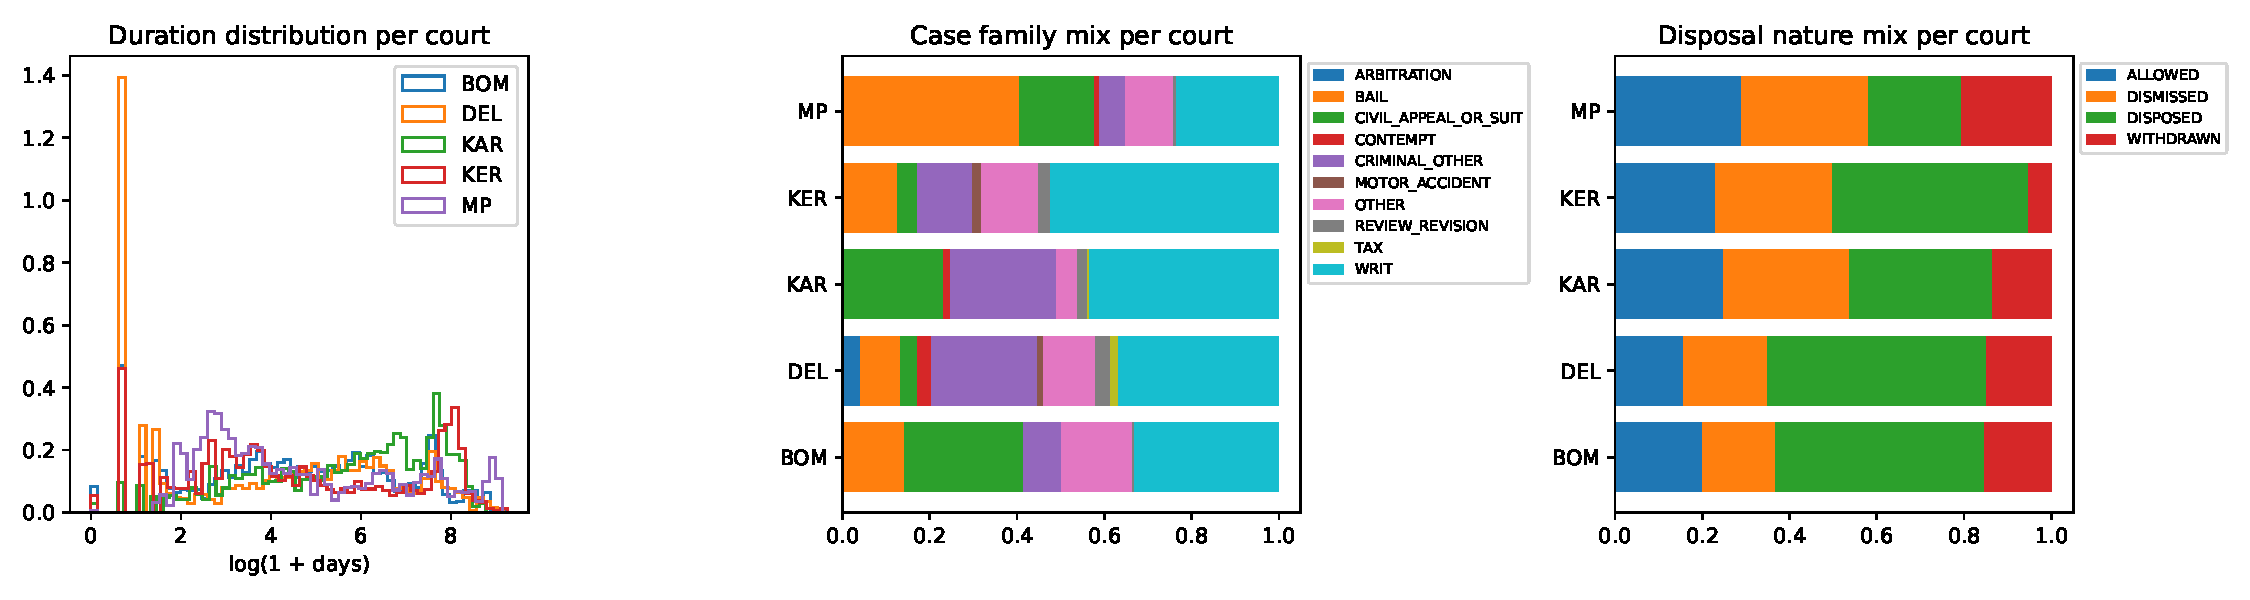
\includegraphics[width=\linewidth]{fig_heterogeneity.pdf}
\caption{Per-court distributions of case duration, case family and disposal nature (text sample).}
\label{fig:hetero}
\end{figure}

Every test is significant, but with this many cases even small differences are, so the effect sizes
carry the argument. They lead to three conclusions.

\paragraph{The label skew is real but moderate.} Case families differ most between courts (Cram\'er's
$V=0.29$): Madhya Pradesh is dominated by bail matters, Kerala by writs. The outcome mix differs less
($V=0.15$). To compare with the synthetic splits used in FL papers, we found the Dirichlet
concentration whose simulated clients lie as far from the pooled label distribution as the real courts
do~\cite{hsu2019fedavgm}. Case families match $\mathrm{Dir}(\alpha\approx1.6)$ per class and disposal
$\mathrm{Dir}(\alpha\approx10)$, while FL benchmarks usually use $\alpha=0.1$--$0.5$. Label imbalance
alone is therefore not why a shared model struggles.

\paragraph{The concept shift is what hurts a shared model.} The same type of case takes a different
time in each court: case family alone explains 2.8\% of the variance in log-duration, and adding the
court and the court$\times$family interaction raises this to 12.7\%. Within a family the outcome mix
still depends on the court (median $V=0.22$; $V=0.35$ for bail). A model trained on one court and
applied to another loses 0.69 \mae{} on duration (a factor of about 2 in days) and 62\% of its
disposal F1.

\paragraph{The inputs differ too.} After masking places, numbers and dates, the court of a judgment can
be identified with 99.97\% balanced accuracy. Most of the telling features are drafting conventions:
``through Mr'' and ``coram'' in Delhi, ``by Sri'' and ``praying'' in Karnataka, ``the honourable'' and
``aged \ldots\ years'' in Kerala, ``by Shri'' in Madhya Pradesh, ``of judicature at'' in Bombay. A few
are residual identifiers such as bench abbreviations, so the figure is an upper bound on the pure
difference in style.

These results predict which parts of a model should be shared. Case type is coded and drafted in a
court-specific way, so its prediction head should stay local. Duration depends on the court even for
the same case type, so it needs a shared encoder with a court-aware head. Section~\ref{sec:learned}
shows that the learned mixing weights recover this ordering.

% =====================================================================================
\section{Method}
\subsection{Federated setup}
Each court $k$ is a client holding $n_k$ training judgments that never leave it. In each round $t$
every court starts from the global model $w^t$, trains for one local epoch and returns $w^t_k$; the
server sets $w^{t+1}=\sum_k \alpha_k w^t_k$ with $\alpha_k=n_k/\sum_j n_j$ for FedAvg. Training runs
for at most 30 rounds with early stopping after 4 rounds without improvement, and the round with the
lowest size-weighted validation loss is kept. The federation is simulated in PyTorch; only adapter and
head parameters are passed to the aggregation step.

\subsection{Model}
The encoder is InLegalBERT~\cite{paul2023inlegalbert}, adapted with LoRA~\cite{hu2022lora} (rank 8 on
the query and value projections) while its own weights stay frozen; a judgment is represented by the
mean of its token embeddings. Three heads follow: an MLP for duration (Huber loss on $y=\log(1+\text{days})$),
a linear case-type classifier, and an MLP for disposal nature that also receives the predicted
case-type probabilities, so that disposal is predicted given the case type. The loss is
\begin{equation}
\mathcal{L} = \mathcal{L}_{\text{Huber}} + 0.5\,\mathcal{L}^{\text{type}}_{\text{CE}} + \mathcal{L}^{\text{disp}}_{\text{CE}},
\end{equation}
with disposal classes weighted by each court's own class frequencies. Only the LoRA adapters and heads,
about 1\% of the parameters, are exchanged with the server.

\paragraph{Task-specific reading (TSR).} Judgments are long, and a 256-token input forces a choice
between the start (parties, case type, facts) and the end (the reasoning leading to the outcome). TSR
encodes the first and the last 256 tokens separately with the shared encoder, giving $e_{\text{start}}$
and $e_{\text{end}}$, and lets each task $t$ learn its own weighting:
\begin{equation}
w_{t,s} = \operatorname{softmax}_{s}\!\left(\frac{q_t^\top e_s}{\sqrt{H}}\right), \qquad
r_t = \sum_{s\in\{\text{start},\,\text{end}\}} w_{t,s}\, e_s ,
\end{equation}
where $H$ is the hidden size and the queries $q_t$ start at zero (equal weights) and are averaged with
the rest of the shared model. All federated comparisons in Section~\ref{sec:results} use this input.

\paragraph{Per-task learned mixing (PTM).} Section~\ref{sec:hetero} suggests that whether a head should
be shared depends on the task. In PTM every court $k$ keeps, for each task $t$, both the shared head
$g_t$ and its own head $g^{(k)}_t$, and learns how much to trust each:
\begin{equation}
f^{(k)}_t(r_t) = a_{k,t}\, g_t(r_t) + \bigl(1-a_{k,t}\bigr)\, g^{(k)}_t(r_t), \qquad a_{k,t}=\sigma(\alpha_{k,t}),
\end{equation}
with $\alpha_{k,t}$ initialised at 0 ($a_{k,t}=0.5$). The server averages only the shared heads; the
court's own heads and weights never leave it. After federated training each court fine-tunes the model
for one epoch on its own data (+ft). The TSR queries and PTM weights use a learning rate of $10^{-2}$.

\subsection{Baselines}
\begin{itemize}
  \item \textbf{No collaboration:} local training, where each court trains alone.
  \item \textbf{Centralized} training on the pooled data of all courts, not private; this is the
        setting of IL-TUR-style models. We also fine-tune it per court (\textbf{centralized + ft}), the
        strongest non-private competitor.
  \item \textbf{One shared federated model}, the kind of algorithms benchmarked in FedLegal:
        FedAvg~\cite{mcmahan2017communication}, FedProx~\cite{li2020federated} ($\mu=0.01$),
        FedAdam~\cite{reddi2021adaptive} (server learning rate $3\times10^{-3}$) and
        SCAFFOLD~\cite{karimireddy2020scaffold}.
  \item \textbf{Personalised federated models:} FedPer~\cite{arivazhagan2019fedper} (all heads local)
        and Ditto~\cite{li2021ditto}, with $\lambda\in\{0.01, 0.1, 1\}$ chosen on validation loss
        ($\lambda=1$).
\end{itemize}
All methods use the same encoder, TSR input, learning rate ($5\times10^{-4}$), rounds and early stopping.

\subsection{Evaluation}
We report one primary metric per task, computed per court on the temporally later test split and
averaged over courts:
\begin{itemize}
  \item \textbf{Duration: \mae{}}, the mean absolute error on $\log(1+\text{days})$. It is a relative
        error (0.5 means predictions are off by a factor $e^{0.5}\approx1.65$ in days), so a 30-day
        bail matter and a five-year appeal count equally; it is not dominated by the long tail (up to
        about 10,000 days) and it matches the training loss. Spearman correlation only measures
        ranking, and F1 over duration classes depends on arbitrary class edges, so neither is used
        to rank methods.
  \item \textbf{Case type and disposal nature: macro-F1.} The classes are imbalanced and their mix
        differs by court, so accuracy would reward predicting each court's majority class.
\end{itemize}
To rank methods by a single number we use the multi-task measure $\dmtl$~\cite{maninis2019attentive,vandenhende2021mtl},
the mean relative improvement over local training across the three tasks:
\begin{equation}
\dmtl = \frac{100}{3}\sum_{t=1}^{3} s_t\,\frac{M_t - M_t^{\text{local}}}{M_t^{\text{local}}},\qquad
s_t=-1 \text{ for \mae{}},\; +1 \text{ for F1}.
\end{equation}
Local training is the reference because it answers the question each court faces: is joining the
federation better than training alone? We report $\dmtl$ for the mean over courts and for the
\textbf{worst court}, since a federation that helps on average but hurts one member is not acceptable to
that member. Main comparisons use three seeds; significance is tested with Wilcoxon signed-rank tests
over the 15 (court, seed) pairs and with a case-level paired bootstrap within each court. Encoder,
learning rate, truncation, Ditto's $\lambda$ and best round are chosen on validation loss only.
Repeated GPU runs with the same seed differed by up to about 0.02 \mae{}. Experiments ran on Kaggle
(two T4 GPUs).

% =====================================================================================
\section{Results}
\label{sec:results}

\subsection{Encoder and input}
Table~\ref{tab:setting} fixes the setting with FedAvg. InLegalBERT is better than RoBERTa-base~\cite{liu2019roberta}
and a learning rate of $5\times10^{-4}$ is better than $2\times10^{-4}$. The first 256 tokens give the
lowest duration error, while the first and last 128 tokens give much better disposal F1 (0.542 against
0.486) and the lower validation loss. This trade-off between the start and the end of a judgment
motivated TSR.

\begin{table}[H]\centering\small
\resizebox{\linewidth}{!}{\begin{tabular}{@{}llllcccc@{}}\toprule
Encoder & LR & Tokens & Val.\ loss$\downarrow$ & \mae{}$\downarrow$ & Spearman$\uparrow$ & Disp.\ F1$\uparrow$ & Worst \mae{}$\downarrow$ \\ \midrule
InLegalBERT & $2\times10^{-4}$ & first 256 & 2.260 & 1.449 & 0.610 & 0.481 & 1.720 \\
InLegalBERT & $5\times10^{-4}$ & first 256 & 2.226 & \textbf{1.431} & \textbf{0.611} & 0.486 & 1.759 \\
InLegalBERT & $5\times10^{-4}$ & first + last 128 & \textbf{2.164} & 1.460 & 0.599 & 0.542 & 1.886 \\
RoBERTa-base & $2\times10^{-4}$ & first 256 & 2.419 & 1.505 & 0.590 & 0.462 & 1.802 \\
RoBERTa-base & $5\times10^{-4}$ & first 256 & 2.238 & 1.436 & 0.591 & 0.471 & 1.703 \\
RoBERTa-base & $5\times10^{-4}$ & first + last 128 & 2.173 & 1.553 & 0.549 & \textbf{0.547} & 1.968 \\ \bottomrule
\end{tabular}}
\caption{Setting selection with FedAvg (seed 0, single view). Chosen on validation loss.}
\label{tab:setting}
\end{table}

\subsection{Main comparison}
Table~\ref{tab:main} compares all methods with the same TSR model and three seeds.

\begin{table}[H]\centering\small
\setlength{\tabcolsep}{5pt}
\begin{tabular}{@{}lcccccc@{}}\toprule
Method & \mae{}$\downarrow$ & Type F1$\uparrow$ & Disp.\ F1$\uparrow$ & $\dmtl$ (\%)$\uparrow$ & Worst court (\%)$\uparrow$ & $p$ vs ours \\ \midrule
\multicolumn{7}{@{}l}{\emph{No collaboration}} \\
Local only & 1.371 & 0.873 & 0.533 & 0.00 & 0.00 & 0.015 \\ \midrule
\multicolumn{7}{@{}l}{\emph{Federated, one shared model (FedLegal-style)}} \\
FedAvg$^\dagger$ & 1.347 & 0.844 & 0.539 & $-0.15$ & -- & -- \\
FedProx & 1.383 & 0.775 & 0.532 & $-4.05$ & $-9.26$ & $<0.001$ \\
FedAdam & 1.369 & 0.792 & 0.526 & $-3.44$ & $-6.94$ & $<0.001$ \\ \midrule
\multicolumn{7}{@{}l}{\emph{Federated, personalised}} \\
FedPer (all heads local) & 1.375 & 0.913 & 0.556 & $+2.86$ & $-1.99$ & 0.17 \\
Ditto ($\lambda=1$) & \textbf{1.329} & 0.872 & 0.555 & $+2.40$ & $-0.29$ & 0.15 \\
PTM, before fine-tuning & 1.376 & 0.914 & 0.556 & $+2.93$ & $-0.93$ & 0.21 \\
\textbf{PTM + ft (ours)} & 1.359 & \textbf{0.917} & 0.559 & $+3.60$ & $+0.62$ & -- \\ \midrule
\multicolumn{7}{@{}l}{\emph{Centralized (pooled data; not private)}} \\
Centralized & 1.358 & 0.860 & 0.559 & $+1.48$ & $-3.92$ & -- \\
Centralized + ft & 1.333 & 0.906 & \textbf{0.568} & $\mathbf{+4.42}$ & $\mathbf{+1.31}$ & 0.30 \\ \bottomrule
\end{tabular}
\caption{Main comparison: TSR input, InLegalBERT + LoRA, 3 seeds, test set, mean over courts.
$\dmtl$ relative to local training; worst court is the lowest per-court $\dmtl$; $p$: Wilcoxon over 15
(court, seed) pairs. $^\dagger$Earlier runs (3 seeds) not repeated in the final batch; $\dmtl$ computed
against the same local reference. SCAFFOLD diverged ($\dmtl=-37\%$) with our AdamW local optimizer,
whose adaptive steps break SCAFFOLD's SGD-based drift correction, and is not shown.}
\label{tab:main}
\end{table}

\paragraph{Standard federated algorithms do not help.} FedAvg ties local training ($-0.15\%$), and
FedProx and FedAdam are 3--4\% \emph{worse}, with their worst court losing 7--9\%. The loss is almost
entirely in case type (F1 0.78--0.84 against 0.87 locally), the task each court codes in its own way.
This reproduces FedLegal's observation that real legal non-IID data hurt standard FL, here with the
cause identified in Section~\ref{sec:hetero}.

\paragraph{Personalised federation beats training alone.} Our method improves on local training by
$\dmtl=+3.6\%$ (Wilcoxon $p=0.015$). The gain is significant for case type ($p=0.012$, better in all
five courts), smaller for disposal ($+0.026$ F1, $p=0.08$) and not significant for duration. Ours is
the only federated method whose worst court also improves ($+0.6\%$), and it beats FedProx and
FedAdam by 9--10\% ($p<0.001$).

\paragraph{The personalised methods are statistically tied.} The differences between ours and FedPer
($p=0.17$) or Ditto ($p=0.15$) are not significant. Ditto has the lowest duration error and ours the
best case-type F1. What PTM adds over them is not accuracy but interpretable sharing weights
(Section~\ref{sec:learned}), learned in one training stage.

\paragraph{Federation matches centralized training.} Pooling all data and fine-tuning per court is
0.6\% ahead of ours, which is not significant (Wilcoxon $p=0.30$; the case-level bootstrap 95\%
intervals of the difference include zero for every metric in each seed). Plain centralized training
is 2.1\% \emph{behind} ours, because one pooled model does not fit any court well. Federation thus
reaches centralized-level accuracy while every judgment stays in its court.

\paragraph{Per court.} Table~\ref{tab:percourt} shows that the gains are largest where local training
is weakest. Bombay, the hardest court for case type and disposal, gains most from federation: case-type
F1 rises from 0.605 to 0.722 and disposal F1 from 0.434 to 0.509.

\begin{table}[H]\centering\small
\setlength{\tabcolsep}{4.5pt}
\begin{tabular}{@{}l ccc ccc ccc@{}}\toprule
 & \multicolumn{3}{c}{\mae{}$\downarrow$} & \multicolumn{3}{c}{Type F1$\uparrow$} & \multicolumn{3}{c}{Disp.\ F1$\uparrow$} \\
\cmidrule(lr){2-4}\cmidrule(lr){5-7}\cmidrule(lr){8-10}
Court & Local & Ours & Cent.+ft & Local & Ours & Cent.+ft & Local & Ours & Cent.+ft \\ \midrule
Bombay & 1.561 & 1.553 & 1.493 & 0.605 & \textbf{0.722} & 0.696 & 0.434 & \textbf{0.509} & 0.500 \\
Delhi & 1.711 & 1.734 & 1.697 & 0.928 & \textbf{0.946} & 0.941 & 0.558 & 0.565 & 0.569 \\
Karnataka & 1.330 & 1.293 & 1.276 & 0.976 & 0.985 & 0.988 & 0.471 & 0.523 & 0.531 \\
Kerala & 1.184 & \textbf{1.166} & 1.181 & 0.874 & 0.946 & 0.963 & 0.479 & 0.469 & 0.498 \\
Madhya Pradesh & 1.071 & 1.047 & 1.017 & 0.981 & 0.983 & 0.941 & 0.722 & 0.726 & 0.743 \\ \bottomrule
\end{tabular}
\caption{Per-court test results, mean over 3 seeds. Bold: ours best of the three.}
\label{tab:percourt}
\end{table}

\subsection{Is TSR more than extra context?}
TSR reads $2\times256$ tokens, while the single-view baselines of earlier versions read 256. A
single-view model reading the first and last 256 tokens (512 in total) separates the two effects
(Table~\ref{tab:control}). It does as well as TSR: local training at 512 tokens reaches \mae{} 1.347
and $\dmtl=+3.7\%$, statistically tied with ours ($p=0.98$), and FedAvg + ft at 512 tokens gives
$+3.2\%$ ($p=0.33$). The duration improvement we attributed to TSR in the mid-term report therefore
comes mostly from reading more of the judgment rather than from the task-specific weighting. The
federated pattern is the same at 512 tokens: plain FedAvg loses on case type ($-3.2\%$) and per-court
fine-tuning recovers it.

\begin{table}[H]\centering\small
\begin{tabular}{@{}llccccc@{}}\toprule
Input & Method & \mae{}$\downarrow$ & Type F1$\uparrow$ & Disp.\ F1$\uparrow$ & $\dmtl$ (\%) & Worst court (\%) \\ \midrule
Single view, 256 & FedAvg & 1.469 & 0.777 & 0.534 & $-5.95$ & $-11.07$ \\
Single view, 256 & FedAvg + ft & 1.474 & 0.905 & 0.552 & $-0.04$ & $-7.08$ \\ \midrule
Single view, 512 & Local & 1.347 & 0.901 & 0.565 & $+3.71$ & $-0.61$ \\
Single view, 512 & Centralized & \textbf{1.332} & 0.875 & \textbf{0.572} & $+3.47$ & $-1.13$ \\
Single view, 512 & FedAvg & 1.359 & 0.757 & 0.549 & $-3.15$ & $-9.08$ \\
Single view, 512 & FedAvg + ft & 1.367 & 0.901 & 0.565 & $+3.21$ & $+0.05$ \\ \midrule
TSR, $2\times256$ & PTM + ft (ours) & 1.359 & \textbf{0.917} & 0.559 & $+3.60$ & $+0.62$ \\ \bottomrule
\end{tabular}
\caption{Effect of the input. $\dmtl$ relative to local training with TSR (Table~\ref{tab:main}); 3 seeds.}
\label{tab:control}
\end{table}

\subsection{What the model learned}
\label{sec:learned}
\paragraph{Where each task reads.} Figure~\ref{fig:segw} shows the learned TSR attention on the end of
the judgment. The pattern is the same in every court and under federated, local and centralized
training: case type reads mainly the start (13--25\% on the end), where the petition type appears;
disposal nature reads mainly the end (65--86\%), where the reasoning leading to the outcome is; duration
uses both (49--72\%).

\begin{figure}[H]\centering
\includegraphics[width=0.9\linewidth]{fig_segment_weights.pdf}
\caption{TSR: share of attention on the end of the judgment per court and task (0.5 = equal).}
\label{fig:segw}
\end{figure}

\paragraph{How much each court relies on the shared heads.} Figure~\ref{fig:mixw} shows the PTM weights
on the shared head. They are stable across seeds and order the tasks the same way in every court:
duration 0.34--0.44, disposal 0.15--0.20 and case type 0.04--0.08. Courts rely on collaboration most for
duration and hardly at all for case type, as predicted by the heterogeneity tests. A fixed
experiment confirms this: with a single-view model, keeping the case-type head local raises its F1 from
0.774 to 0.919, while keeping the duration head local raises the duration error from 1.474 to 1.494.
Kerala relies most on the shared duration head (0.44) and Bombay least (0.34).

\begin{figure}[H]\centering
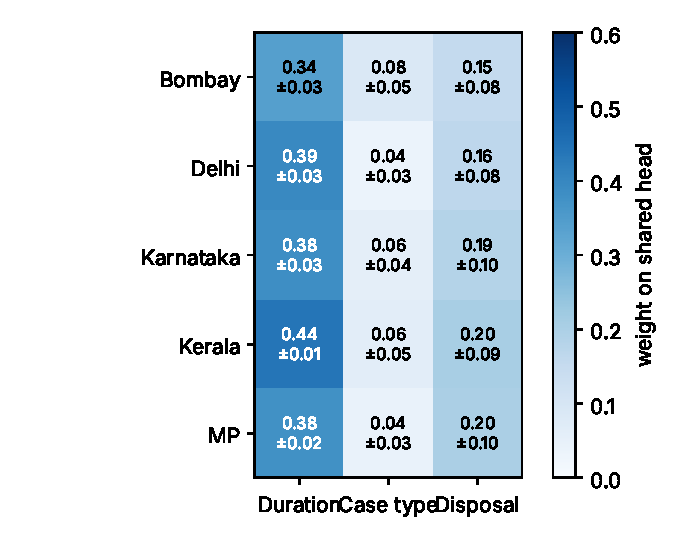
\includegraphics[width=0.62\linewidth]{fig_mixing_weights.pdf}
\caption{PTM: learned weight on the shared head per court and task (1 = shared only, 0 = own head only),
mean $\pm$ std over 3 seeds.}
\label{fig:mixw}
\end{figure}

\subsection{What federation gives a court}
\paragraph{Courts with little data.} Each court keeps only 10\%, 25\% or 50\% of its training judgments
(about 175, 440 and 875 cases; one seed; Table~\ref{tab:lowres} and Figure~\ref{fig:flhelps}a).
Federation helps most when a court has a few hundred cases: at 25\% it raises case-type F1 from 0.63 to
0.81 and gives $\dmtl=+7.3\%$, about two thirds of what pooling the raw data gives. With very little data
(10\%) the gain is mostly in case type, duration becomes worse than local training (1.70 against 1.60),
and pooled training is far ahead. With half the data the gain falls to $+1.4\%$. These are single-seed
results and indicate a trend.

\begin{table}[H]\centering\small
\resizebox{\linewidth}{!}{\begin{tabular}{@{}lcccc@{}}\toprule
Data per court & Local \mae{} / type F1 & Federated \mae{} / type F1 & Federated $\dmtl$ (\%) & Centralized $\dmtl$ (\%) \\ \midrule
10\% & 1.599 / 0.523 & 1.704 / 0.598 & $+2.3$ & $+12.2$ \\
25\% & 1.487 / 0.626 & 1.555 / 0.812 & $+7.3$ & $+10.7$ \\
50\% & 1.403 / 0.808 & 1.439 / 0.881 & $+1.4$ & $-0.8$ \\
100\% (3 seeds) & 1.371 / 0.873 & 1.359 / 0.917 & $+3.6$ & $+1.5$ \\ \bottomrule
\end{tabular}}
\caption{Federated (PTM + ft) and centralized training against local training as data shrink.
$\dmtl$ relative to local training with the same data. One seed except the last row.}
\label{tab:lowres}
\end{table}

\paragraph{A court with no labelled data.} Each court in turn is left out of training and only evaluated
(Table~\ref{tab:unseen}, Figure~\ref{fig:flhelps}b). Without federation it could only borrow another
court's model. For four of five courts, the federated model trained on the other four is the best
available option: better than the best single other court (chosen with hindsight on the test set) and
better than centralized training on the same four courts. The exception is Madhya Pradesh, whose
bail-dominated caseload is the most unusual. Every option is still 16--44\% below the court's own local
model, so a new court should join the federation and fine-tune rather than use the shared model as is.

\begin{table}[H]\centering\small
\begin{tabular}{@{}lcccc@{}}\toprule
Held-out court & Mean other court & Best other court & Federated, 4 courts & Centralized, 4 courts \\ \midrule
Bombay & $-36.0$ & $-31.3$ & $\mathbf{-25.9}$ & $-28.9$ \\
Delhi & $-49.2$ & $-42.5$ & $\mathbf{-37.7}$ & $-39.0$ \\
Karnataka & $-35.1$ & $-17.3$ & $\mathbf{-15.6}$ & $-30.4$ \\
Kerala & $-52.9$ & $-42.4$ & $\mathbf{-32.8}$ & $-40.8$ \\
Madhya Pradesh & $-51.0$ & $\mathbf{-41.3}$ & $-43.6$ & $-46.0$ \\ \bottomrule
\end{tabular}
\caption{Unseen court: $\dmtl$ (\%) relative to the court's own local model (one seed).}
\label{tab:unseen}
\end{table}

\begin{figure}[H]\centering
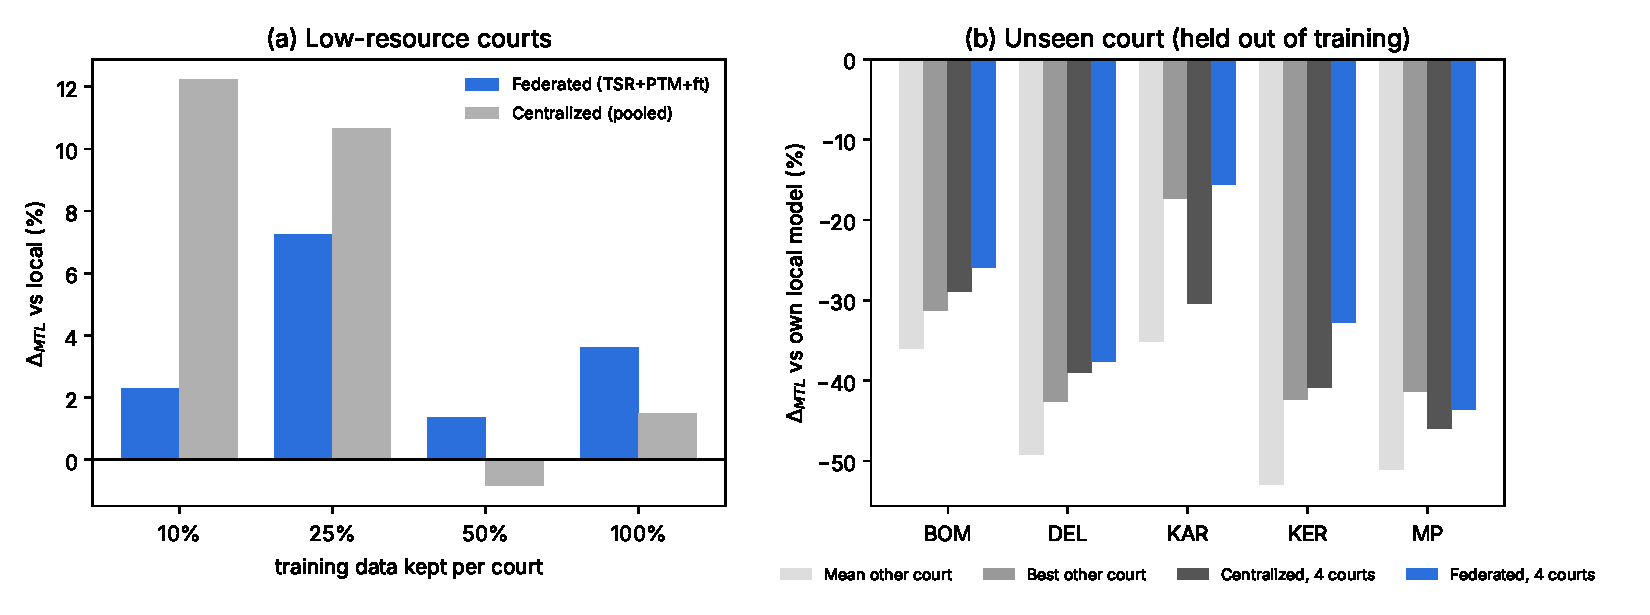
\includegraphics[width=\linewidth]{fig_flhelps.pdf}
\caption{(a) Gain over local training when every court keeps only part of its data. (b) Performance on a
court left out of training, relative to that court's own local model.}
\label{fig:flhelps}
\end{figure}

% =====================================================================================
\section{Discussion}
\paragraph{RQ1: heterogeneity.} The five courts are significantly non-IID in every respect tested. The
label mix differs only moderately; the courts differ most in how the same type of case behaves
(duration and outcome given case type) and in how judgments are written. This explains which parts of a
model can be shared, and the learned sharing weights agree with it.

\paragraph{RQ2: federated against local and centralized training.} Standard federated algorithms do not
beat local training on these courts, and FedProx and FedAdam are worse; the aggregation rule matters
much less than what is personalised. With per-task personalisation, federated training beats local
training ($p=0.015$), improves the worst court, beats FedLegal-style algorithms by 9--10\%, ties the
personalised methods FedPer and Ditto, and is statistically tied with the best centralized model.

\paragraph{Why federate if centralized training exists?} Centralized models such as those benchmarked in
IL-TUR need all courts' records in one place. When that is not allowed, the realistic alternative is
training alone, and federation beats it. When it is allowed, it buys little: centralized training with
per-court fine-tuning is only 0.6\% ahead (not significant), and without fine-tuning it is behind.
Federation also gives courts with a few hundred cases a large gain, and gives a new court a better
starting model than borrowing another court's model.

\paragraph{RQ3: generalisation and privacy.} All results are on each court's temporally later cases. A
court that never trained gets a usable but clearly weaker model, so new courts should fine-tune. Only
LoRA adapters and heads (about 1\% of the model) leave a court, and with PTM the court's own heads and
weights never leave it. Model updates can still leak information, and secure
aggregation~\cite{bonawitz2017secagg} and differential privacy~\cite{mcmahan2018dp} have not been
applied, so no formal privacy guarantee is claimed.

\paragraph{Limitations.} The data are public judgments of cases decided in 2024; the privacy motivation
concerns deployment on confidential pre-filing material, which we could not test. Labels for case type
and disposal are rule-based. The low-resource and unseen-court experiments use one seed. GPU runs were
not exactly reproducible (up to about 0.02 \mae{}). SCAFFOLD was run with an AdamW local optimizer and
diverged; an SGD-based run would be a fairer test. The court-identification accuracy is an upper bound
on style differences because some identifiers survive masking.

\paragraph{Future work.} Secure aggregation and client-level differential privacy would turn the privacy
argument into a measured guarantee. More courts and decision years, survival models that can use
pending cases, and further seeds for the low-resource and unseen-court experiments would strengthen the
conclusions.

\section{Conclusion}
Indian High Courts are measurably non-IID, mainly in how the same kind of case behaves and in how
judgments are written. Standard federated learning does not overcome this. Federated learning with
per-task personalisation does: it beats training alone, protects the hardest court, and matches
centralized training on pooled data without moving any judgment. It helps most for courts with few
labelled cases, and its learned weights show that courts gain from sharing most for case duration and
hardly at all for case type.

% =====================================================================================
\begin{thebibliography}{99}\small
\bibitem{arivazhagan2019fedper} M.~G. Arivazhagan, V.~Aggarwal, A.~K. Singh, and S.~Choudhary. Federated learning with personalization layers. \emph{arXiv:1912.00818}, 2019.
\bibitem{bonawitz2017secagg} K.~Bonawitz et al. Practical secure aggregation for privacy-preserving machine learning. In \emph{ACM CCS}, 2017.
\bibitem{collins2021fedrep} L.~Collins, H.~Hassani, A.~Mokhtari, and S.~Shakkottai. Exploiting shared representations for personalized federated learning. In \emph{ICML}, 2021.
\bibitem{dattam_hc} Dattam Labs. Indian High Court Judgments. Registry of Open Data on AWS, CC-BY-4.0, 2025.
\bibitem{deng2020apfl} Y.~Deng, M.~M. Kamani, and M.~Mahdavi. Adaptive personalized federated learning. \emph{arXiv:2003.13461}, 2020.
\bibitem{hsu2019fedavgm} T.-M.~H. Hsu, H.~Qi, and M.~Brown. Measuring the effects of non-identical data distribution for federated visual classification. \emph{arXiv:1909.06335}, 2019.
\bibitem{hu2022lora} E.~J. Hu et al. LoRA: Low-rank adaptation of large language models. In \emph{ICLR}, 2022.
\bibitem{joshi2024iltur} A.~Joshi, S.~Paul, A.~Sharma, P.~Goyal, S.~Ghosh, and A.~Modi. IL-TUR: Benchmark for Indian legal text understanding and reasoning. In \emph{ACL}, 2024.
\bibitem{kairouz2021advances} P.~Kairouz, H.~B. McMahan, et al. Advances and open problems in federated learning. \emph{Foundations and Trends in Machine Learning}, 14(1--2):1--210, 2021.
\bibitem{kalamkar2022ner} P.~Kalamkar, A.~Agarwal, A.~Tiwari, S.~Gupta, S.~Karn, and V.~Raghavan. Named entity recognition in Indian court judgments. In \emph{NLLP Workshop}, 2022.
\bibitem{karimireddy2020scaffold} S.~P. Karimireddy, S.~Kale, M.~Mohri, S.~Reddi, S.~Stich, and A.~T. Suresh. SCAFFOLD: Stochastic controlled averaging for federated learning. In \emph{ICML}, 2020.
\bibitem{fedlbw2026} M.~Kundroo, T.~Singh, and T.~Kim. FedLBW: A loss-based weighting strategy for federated learning on non-IID data in wireless networks. \emph{Expert Systems with Applications}, 302:130487, 2026.
\bibitem{li2020federated} T.~Li, A.~K. Sahu, M.~Zaheer, M.~Sanjabi, A.~Talwalkar, and V.~Smith. Federated optimization in heterogeneous networks. In \emph{MLSys}, 2020.
\bibitem{li2020qffl} T.~Li, M.~Sanjabi, A.~Beirami, and V.~Smith. Fair resource allocation in federated learning. In \emph{ICLR}, 2020.
\bibitem{li2021ditto} T.~Li, S.~Hu, A.~Beirami, and V.~Smith. Ditto: Fair and robust federated learning through personalization. In \emph{ICML}, 2021.
\bibitem{liu2019roberta} Y.~Liu et al. RoBERTa: A robustly optimized BERT pretraining approach. \emph{arXiv:1907.11692}, 2019.
\bibitem{lopezpaz2017c2st} D.~Lopez-Paz and M.~Oquab. Revisiting classifier two-sample tests. In \emph{ICLR}, 2017.
\bibitem{lu2024fedhca2} Y.~Lu et al. FedHCA$^2$: Towards hetero-client federated multi-task learning. In \emph{CVPR}, 2024.
\bibitem{maninis2019attentive} K.-K. Maninis, I.~Radosavovic, and I.~Kokkinos. Attentive single-tasking of multiple tasks. In \emph{CVPR}, 2019.
\bibitem{mcmahan2017communication} B.~McMahan, E.~Moore, D.~Ramage, S.~Hampson, and B.~Ag\"uera y Arcas. Communication-efficient learning of deep networks from decentralized data. In \emph{AISTATS}, 2017.
\bibitem{mcmahan2018dp} H.~B. McMahan, D.~Ramage, K.~Talwar, and L.~Zhang. Learning differentially private recurrent language models. In \emph{ICLR}, 2018.
\bibitem{njdg} National Judicial Data Grid. eCourts Services, Government of India. \url{https://njdg.ecourts.gov.in}, accessed October 2026.
\bibitem{nigam2025nyayarag} S.~K. Nigam et al. NyayaRAG: Realistic legal judgment prediction with RAG under the Indian common law system. In \emph{IJCNLP-AACL}, 2025.
\bibitem{paul2022lesicin} S.~Paul, P.~Goyal, and S.~Ghosh. LeSICiN: A heterogeneous graph-based approach for automatic legal statute identification from Indian legal documents. In \emph{AAAI}, 2022.
\bibitem{paul2023inlegalbert} S.~Paul, A.~Mandal, P.~Goyal, and S.~Ghosh. Pre-trained language models for the legal domain: A case study on Indian law. In \emph{ICAIL}, 2023.
\bibitem{reddi2021adaptive} S.~J. Reddi et al. Adaptive federated optimization. In \emph{ICLR}, 2021.
\bibitem{taskawarefl2025} Task-aware federated multi-task learning. In \emph{ACM Multimedia Asia}, 2025.
\bibitem{vandenhende2021mtl} S.~Vandenhende, S.~Georgoulis, W.~Van~Gansbeke, M.~Proesmans, D.~Dai, and L.~Van~Gool. Multi-task learning for dense prediction tasks: A survey. \emph{IEEE TPAMI}, 2021.
\bibitem{vats2023llms} S.~Vats et al. LLMs -- the good, the bad or the indispensable?: A use case on legal statute prediction and legal judgment prediction on Indian court cases. In \emph{Findings of EMNLP}, 2023.
\bibitem{yue2023fedjudge} L.~Yue, Q.~Liu, Y.~Du, W.~Gao, Y.~Liu, and F.~Yao. FedJudge: Federated legal large language model. \emph{arXiv:2309.08173}, 2023.
\bibitem{zhang2023fedala} J.~Zhang et al. FedALA: Adaptive local aggregation for personalized federated learning. In \emph{AAAI}, 2023.
\bibitem{zhang2023fedlegal} Z.~Zhang, X.~Hu, J.~Zhang, Y.~Zhang, H.~Wang, L.~Qu, and Z.~Xu. FEDLEGAL: The first real-world federated learning benchmark for legal NLP. In \emph{ACL}, 2023.
\end{thebibliography}

\end{document}
